\begin{frame}{Ausblick}
	\begin{itemize}
	\uncover<2->{
		\item Einbindung des RF-Data-Tools zur Beurteilung der Qualität des Ausgangssignals
		}
		\uncover<3->{
		\item \textit{Zusatz:} Konvertierung der Funktionalitäten von Python in die TEMF RF-Data-Tools
		}
	\end{itemize}
\end{frame}

\begin{frame}{Ausblick}
	
	\begin{itemize}
		\item Optimierung der linearen Übertragungsfunktion: %mittels Auswertung der erwarteten und gemessenen Ausgangssignale $U_{out}$: 
		\begin{align*}
			\underline{H}^{\mathrm{neu}} \left( \omega \right) = \underline{H}^{\mathrm{alt}} \left( \omega \right) \left( 1+ \sigma_H \cdot \left( \frac{\underline{U}_{out,\mathrm{mess}}\left( \omega \right) }{\underline{U}_{out,\mathrm{ideal}} \left( \omega \right) } -1 \right) \right) 
		\end{align*}
		mit $ \sigma_H $ als Schrittweite. %der jeweiligen Iteration
		% würde Notation als Vektoreintrag vorschlagen H_{...} [i] statt Darstellung als Funktion
		
	\end{itemize}

	
	\begin{picture}(100,70)
		\put(15,-10){
			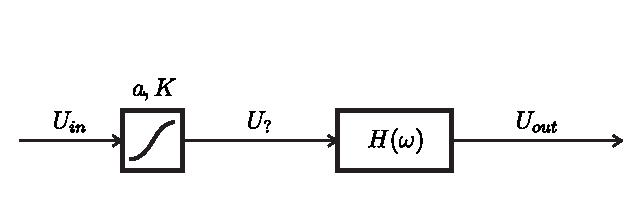
\includegraphics[scale=1.0]{slides/ResultCode/Slide1.eps} 
		}
	\end{picture}
\end{frame}
	
%%%%%%% weitere Kommentare: %%%%%%%%%%%%%%
%Frequenzverhalten der Kennlinie? Funktioniert Optimierung wie angesprochen überhaupt sinnvoll?
% mit welcher Iteration? Zuerst H optimieren, dann neue Werte generieren (messen) und dann K? Oder beides nacheinander und dann erst neu messen?
\begin{frame}{Ausblick}
	
	\begin{itemize}
		\item Optimierung der nichtlinearen Kennlinie: %mittels Vergleich der Differenz der erwarteten und gemessenen Spannungssignale $U_{quest}$ und der Faktoren $a$ der polynomialen Kennlinie:
		\begin{align*}
			\Delta U_{?} = U_{?, \mathrm{mess}} - U_{?, \mathrm{berechnet}} = \sum_n \tilde{a}_n U_{in}^n
			&&
			a_n^{\mathrm{neu}} = a_n^{\mathrm{alt}} + \sigma_a \cdot \tilde{a}_n
		\end{align*}
		mit $\sigma_a$ als Schrittweite. %der jeweiligen Iteration
	\end{itemize}
	
	\begin{picture}(100,70)
		\put(15,-10){
			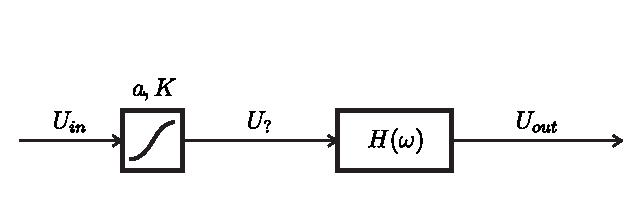
\includegraphics[scale=1.0]{slides/ResultCode/Slide1.eps} 
		}
	\end{picture}



\end{frame}





